
\section{Below threshold measures}
Below threshold measures, \BTM, can be defined as
\begin{equation}
    \BTM^{(p)}_\alpha = \left\| \left(\alpha - r\right)^+ \right\|_p,
    \label{btm1}
\end{equation}
where $\alpha \in \mR$ is the threshold and $\|\cdot\|_p = (\mE[|\cdot|^p])^{1/p}$ is the $L^p$-norm.

The most popular members of \BTM\ family are the \BTAD, Below Threshold Absolute Deviation, for $p=1$, and
\BTSD, Below Threshold Semi-Deviation, for $p=2$. However, famous are their corresponding generalized Sharpe ratios.
For $\mu_0=\alpha$,
\begin{itemize}
  \item \BTAD-Sharpe ratio is the Omega ratio,
  \item \BTSD-Sharpe ratio  is the Sortino ratio.
\end{itemize}
Both, Omega and Sortino optimal portfolio strategies are popular among practitioners.

In general, \BTM\ can be defined in terms of both standard rates of return $r$, as in Eq.~(\ref{btm1}), and
detrended rates of return, by replacing $r$ with $\br = r - \mE[r]$.
Expressed in terms of detrended rate of return and for $\alpha=0$, $\BTAD_0$ is equivalent to the first level \mMAD, $\delta^{(1)}_1$ from Eq.~(\ref{mmad0}),
while $\BTSD_0$ to the first level \mLSD, $\delta^{(2)}_1$ from Eq.~(\ref{LSD0}). In general, $\BTM^{(p)}_0$ (\ie\ for $\alpha=0$) with detrended rate of returns,
is equivalent to the first level $\mHMDD^{(p)}$, $\delta^{(p)}_1$ from Eq.~(\ref{hmdd1}).

Just as in the case of Tail dispersion measures, Eq.~(\ref{qq3}), \BTM\ can be extended to a mixture of $\BTM^{(p)}$ for different thresholds, \ie,
\begin{equation}
    \mBTM^{(p)} = \sum_{l=1}^L \cK_l \times \BTM^{(p)}_{\alpha_l},
    \label{btm2}
\end{equation}
where $\{\cK_l\}_{l=1,\cdots,L}$ is a set of positive mixture coefficients normalized to unit and
$\{\alpha_l\}_{l=1,\cdots,L}$ is a set of distinct thresholds.

Unlike the Tail and Downside measures, $\mBTM^{(p)}$ are not genuine dispersion measures.
They violate the positive homogeneity axiom and, in the case where standard rates of return are used, they also violate the location invariance.
An exception is the case where $L=1$ and $\alpha_1=0$ with detrended rate of return.
In this case $\mBTM^{(p)}$ becomes $\BTM^{(p)}_0$, which is a genuine dispersion measure.

However, the methodologies of optimal portfolio construction outlined in Sec.~\ref{strategies} can formally be applied to \mBTM.
They will be presented for \mBTAD\ (mixture \BTAD) and \mBTSD\ (mixture \BTSD) in the next two sections, respectively.

\BackToContents


\subsection{mBTAD-based optimization strategies}\label{S:mBTAD}

\BTAD\ stands for Below Threshold Absolute Deviation measure and is defined as
\begin{equation}
    \BTAD_\alpha = \mE\left[\left(\alpha - r\right)^+ \right],
    \label{oo1}
\end{equation}
where $\alpha \in \mR$ is called threshold.
The measure has gained in popularity after the introduction of
Omega ratio in 2002 by Keating and Shadwick \cite{Keating}.

Omega ratio is an investment performance measure. It was introduced as an alternative to Sharpe ratio
to measure expected excess return per unit of downside risk of realizations below a predefined threshold.
Over the years it has become very popular among practitioners.
It can be defined as\footnote{In the original paper of Keating and Shadwick \cite{Keating}, Omega ratio is defined without the $-1$.
It is a matter of convenience, adding or subtracting a constant from the ratio will not affect the optimal portfolio
composition. In our case it facilitates a readable expression for Eq.~(\ref{oo3}).}
\begin{equation}
    \Omega_{\mu_0} = \frac{\int_{\mu_0}^{+\infty} [1 - F(r)] dr}{\int_{-\infty}^{\mu_0} F(r) dr} - 1,
    \label{oo2}
\end{equation}
where $\mu_0$ is a constant called Omega threshold and $F(\cdot)$ is the portfolio rate of return cdf.
It is straightforward to show that $\Omega_{\mu_0}$ ratio can be expressed as
\begin{equation}
    \Omega_{\mu_0} = \frac{\mE(r) - \mu_0}{\mE[(\mu_0 - r)^+]}.
    \label{oo3}
\end{equation}
It is clear that the denominator from Eq.~(\ref{oo3}) is $\BTAD_{\mu_0}$. Therefore, Omega ratio can be viewed as
\BTAD-Sharpe ratio for $\alpha=\mu_0$.

As we mentioned in the preamble of this section, \BTAD\ can be defined in terms of both standard rate of return $r$ and
detrended rate of return $\br = r - \mE[r]$. In this subsection we will use the latter specification to write down the mathematical expressions. However, we should keep in
mind that, switching between the \BTAD\ definitions, is a simple matter of replacing $\br$ with $r$.\footnote{\azapy\ package provides a logical
flag to switch between the use of $r$ and $\br$ (see \azapydoc).}

Following the result from  Eq.~(\ref{btm2}), \mBTAD\ is defined as a superposition of \BTAD, \ie,
\begin{equation}
    \mBTAD = \sum_{l=1}^L \cK_l \times \BTAD_{\alpha_l},
    \label{oo0}
\end{equation}
where $\{\cK_l\}_{l=1,\cdots,L}$ is a set of positive constants normalized to unit (the mixture coefficients) and
$\{\alpha_l\}_{l=1,\cdots,L}$ is a set of distinct thresholds.

We will refer to the \mBTAD-Sharpe ratio as Omega ratio, since Omega ratio terminology is used more often among practitioners. However,
we should keep in mind, that our Omega ratio definition is equivalent to the original Keating and Shadwick \cite{Keating}
definition only in the case where $L=1$ and $\alpha_1 = \mu_0$ with standard rate of return.

In general, \mBTAD\ is not a genuine dispersion measure. It violates the positive homogeneity axiom and, in the case where standard rates of return
are used, it also violates local invariance. An exception is the case where $L=1$ and $\alpha_1=0$ with detrended rates of return.
In this case $\BTAD_0$ is equivalent to the first order \mMAD, delta-risk $\delta^{(1)}_1$ from Eq.~(\ref{mmad01}), which is a
genuine dispersion measure.

\BackToContents

\subsubsection{mBTAD dispersion measure}
The computation of the \BTAD\ is straightforward. Given a set $\{r_i\}_{i=1,\cdots,N}$ of observed rates or returns, we have
\begin{equation}
    \BTAD_\alpha = \frac{1}{N}\sum_{i=1}^N (\alpha - \br_i)^+.
    \label{btad01}
\end{equation}
Then, \mBTAD\ is given by the sum from Eq.~(\ref{oo0}).

\BackToContents

\subsubsection{mBTAD optimal portfolio}
The optimization is described by Eqs.~(\ref{gg1}) from Sec.~\ref{strategies} point~\ref{OptRisk},
where $\rho$ is given by \mBTAD\ from Eq.~(\ref{oo0}).
It is the following LP problem.

\bigskip
\noindent Minimize over $\{\{w_k\}_{k=1,\cdots,M}, \{ \eta_l, \{ s_{li} \}_{i=1,\cdots,N} \}_{l=1,\cdots,L} \}$,
\begin{subequations}\label{btad1}
\begin{align}
    &g = \sum_{l=1}^L \cK_l \eta_l, \label{btad1a} \\
    \st & \frac{1}{N} \sum_{i=1}^N s_{li} = \eta_l, \label{btad1b} \\
    & s_{li} + \sum_{k=1}^M w_k \br_{ki} \geq \alpha_l, \label{btad1c} \\
    & \sum_{k=1}^M w_k \mu_k \geq \mu, \label{btad1d} \\
    & \sum_{k=1}^M w_k = 1, \label{btad1e} \\
    & s_{li} \geq 0, \label{btad1g} \\
    & \eta_l \geq 0, \label{btad1h} \\
    & w_k \geq 0, \label{btad1f}
\end{align}
\end{subequations}

\noindent where $\mu$, in Eq.~(\ref{btad1d}), is the portfolio targeted expected rate of return, while $\mu_k$ for $k = 1,\cdots,M$
are the portfolio components expected rate of returns.
Then, we have
\begin{subequations}\label{btad2}
\begin{align}
    \RR &= \sum_{k=1}^M w_k^* \mu_k, \label{btad2a} \\
    \mBTAD &= g^*, \label{btad2b} \\
    \BTAD_{\alpha_l} &= \eta_l^*, \label{btad2c}
\end{align}
\end{subequations}

\noindent where $^*$ denotes the solution of LP problem.
In addition to the optimal portfolio weights $\{w_k^*\}_{k=1,\cdots,M}$ and
expected rate of return $\RR$, the
LP solution provides information about the portfolio \mBTAD\ and its components.

\bigskip
\noindent Here is an example, using the \azapy\ package, of how to compute the \mBTAD\ optimal portfolio.
The \mBTAD\ time horizon was set to one quarter and the calibration is performed using the prior 3.25 years of
close-adjusted historical prices (default settings).
For more details see the package documentation at \azapydoc.

\lstinputlisting[language=Python]{../PyScripts/BTAD_RiskOptim.py}

\BackToContents


\subsubsection{Minimum mBTAD portfolio}

Following the result from Sec.~\ref{strategies} point~\ref{MinRisk},
the algorithm to compute the optimal portfolio with minimum \mBTAD\ is given by Eqs.~(\ref{btad1}) where
$\mu$ from r.h.s. of Eq.~(\ref{btad1d}) is set to a value equal to the smallest expected rate of
return among the portfolio components, \ie\ $\mu=\min_k\{\mu_k\}$.

\bigskip
\noindent Here is an example, using the \azapy\ package, of how to compute the minimum \mBTAD\ portfolio.
The \mBTAD\ time horizon was set to one quarter and the calibration is performed using the prior 3.25 years of
close-adjusted historical prices (default settings).
For more details see the package documentation at \azapydoc.

\lstinputlisting[language=Python]{../PyScripts/BTAD_MinRisk.py}

\BackToContents

\subsubsection{mBTAD optimal portfolio for targeted risk value}
This optimization is described by Eqs.~(\ref{gg2}) from Sec.~\ref{strategies} point~\ref{TargetRisk},
where $\rho$ is given by $\mBTAD$ from Eq.\ (\ref{oo0}).
It is the following LP problem.

\bigskip
\noindent Maximize over $\{\{w_k\}_{k=1,\cdots,M}, \{ \eta_l, \{ s_{li} \}_{i=1,\cdots,N} \}_{l=1,\cdots,L} \}$,
\begin{subequations}\label{btad3}
\begin{align}
    &g = \sum_{k=1}^M w_k \mu_k, \label{btad3a} \\
    \st &\sum_{l=1}^L \cK_l \eta_l = \mBTAD_0, \label{btad3b} \\
    & \frac{1}{N} \sum_{i=1}^N s_{li} = \eta_l, \label{btad3c} \\
    & s_{li} + \sum_{k=1}^M w_k \br_{ki} \geq \alpha_l, \label{btad3d} \\
    & \sum_{k=1}^M w_k = 1, \label{btad3e} \\
    & s_{li} \geq 0, \label{btad3g} \\
    & \eta_l \geq 0, \label{btad3h} \\
    & w_k \geq 0, \label{btad3f}
\end{align}
\end{subequations}

\noindent where $\mBTAD_0$ in Eq.~(\ref{btad3b}) is the portfolio targeted \mBTAD\ dispersion value.
Then, we have
\begin{subequations}\label{btad4}
\begin{align}
    \RR &= g^*, \label{btad4a} \\
    \mBTAD_{\alpha_l} &= \eta_l^*, \label{btad4b}
\end{align}
\end{subequations}

\noindent where $^*$ denotes the solution of LP problem.
In addition to the optimal portfolio weights $\{w_k^*\}_{k=1,\cdots,M}$ and expected rate of return $\RR$,
the LP solution provides information about the $\BTAD_{\alpha_l}$ components of $\mBTAD_0$,
although, this information is likely to be known at the outset.

\bigskip
\noindent Here is an example, using the \azapy\ package, of how to compute the optimal portfolio
with the same \mBTAD\ as the equal weighted portfolio.
The \mBTAD\ time horizon was set to one quarter and the calibration is performed using the prior 3.25 years of
close-adjusted historical prices (default settings).
For more details see the package documentation at \azapydoc.

\lstinputlisting[language=Python]{../PyScripts/BTAD_InvNrisk.py}

\BackToContents

\subsubsection{mBTAD optimal portfolio for fixed risk-aversion factor}
This optimization is described by Eqs.~(\ref{gg3}) from Sec.~\ref{strategies} point~\ref{RiskAverse},
where $\rho$ is given by \mBTAD\ from Eq.~(\ref{oo0}).
It is the following LP problem.

\bigskip
\noindent Maximize over $\{\{w_k\}_{k=1,\cdots,M}, \{ \eta_l, \{ s_{li} \}_{i=1,\cdots,N} \}_{l=1,\cdots,L} \}$,
\begin{subequations}\label{btad5}
\begin{align}
    &g = \sum_{k=1}^M w_k \mu_k - \lambda \sum_{l=1}^L \cK_l \eta_l, \label{btad5a} \\
    \st & \frac{1}{N} \sum_{i=1}^N s_{li} = \eta_l, \label{btad5b} \\
    & s_{li} + \sum_{k=1}^M w_k \br_{ki} \geq \alpha_l, \label{btad5c} \\
    & \sum_{k=1}^M w_k = 1, \label{btad5d} \\
    & s_{li} \geq 0, \label{btad5f} \\
    & \eta_l \geq 0, \label{btad5g} \\
    & w_k \geq 0, \label{btad5e}
\end{align}
\end{subequations}

\noindent where $\lambda$ from Eqs.~(\ref{btad5a}) is the risk-aversion factor.
Then, we have
\begin{subequations}\label{btad6}
\begin{align}
    \RR &= \sum_{k=1}^M w_k^* \mu_k, \label{btad6a} \\
    \mBTAD &= \frac{\RR - g^*}{\lambda}, \label{btad6b} \\
    \BTAD_{\alpha_l} &= \eta_l^*, \label{btad6c}
\end{align}
\end{subequations}

\noindent where $^*$ denotes the solution of LP problem.
In addition to the optimal portfolio weights $\{w_k^*\}_{k=1,\cdots,M}$ and expected rate of return $\RR$,
the LP solution provides information about \mBTAD\ and its \BTAD\ components.

\bigskip
\noindent Here is an example, using the \azapy\ package, of how to compute the optimal portfolio
for a given value of the risk-aversion factor $\lambda$.
The \mBTAD\ time horizon was set to one quarter and the calibration is performed using the prior 3.25 years of
close-adjusted historical prices (default settings).
For more details see the package documentation at \azapydoc.

\lstinputlisting[language=Python]{../PyScripts/BTAD_Averse.py}

\BackToContents

\subsubsection{Omega optimal portfolio - maximization solution}
This optimization targets the maximization of Omega ratio. It is based on the
Eqs.~(\ref{gg4}) from Sec.~\ref{strategies} point~\ref{MaxSharpe}, where $\rho$ is given by \mBTAD\ from Eq.~(\ref{oo0}).
The optimization can be formulated as an LP problem
if Eq.\ (\ref{gg4b}) can be linearized. In our case the linearization is straightforward. Introducing the following
variable transformations $\bw_k = t w_k$, $\bs_{li} = t s_{li}$ and $\bbeta_l = t \eta_l$, the LP
problem can be written as follows.

\bigskip
\noindent Maximize over $\{\{\bw_k\}_{k=1,\cdots,M}, \{ \bbeta_l, \{ \bs_{li} \}_{i=1,\cdots,N} \}_{l=1,\cdots,L}, t \}$,
\begin{subequations}\label{btad7}
\begin{align}
    &g = \sum_{k=1}^M \bw_k \mu_k - \mu_0 t, \label{btad7a} \\
    \st &\sum_{l=1}^L \cK_l \bbeta_l = 1, \label{btad7c} \\
    &\frac{1}{N}\sum_{i=1}^N \bs_{li} = \bbeta_l, \label{btad7b} \\
    &\bs_{li}  + \sum_{k=1}^M \bw_k \br_{ki} - \alpha_l t \geq 0, \label{btad7d} \\
    &\sum_{k=1}^M \bw_k - t = 0, \label{btad7e} \\
    &t \geq 0, \label{btad7h} \\
    &\bs_{li} \geq 0, \label{btad7g} \\
    &\bbeta_l \geq 0, \label{btad7i} \\
    &\bw_k \geq 0, \label{btad7f}
\end{align}
\end{subequations}

\noindent where $\mu_0$ from Eq.~(\ref{btad7a}) is the risk-free rate accessible to the investor.
Then, we have
\begin{subequations}\label{btad8}
\begin{align}
    w_k &= \frac{\bw_k^*}{t^*} , \label{btad8a} \\
    \RR &= \frac{g^*}{t^*} + \mu_0, \label{btad8c} \\
    \Omega &= g^*, \label{btad8b} \\
    \mBTAD &= \frac{1}{t^*}, \label{btad8d} \\
    \BTAD_{\alpha_l} &= \frac{\bbeta_l^*}{t^*}, \label{btad8e}
\end{align}
\end{subequations}

\noindent where $^*$ denotes the solution of LP problem.
In addition to the optimal portfolio weights $\{w_k\}_{k=1,\cdots,M}$, expected rate of return $\RR$ and
Omega ratio $\Omega$,
the solution of LP problem provides information about \mBTAD\ and its components.

\bigskip
\noindent Here is an example, using the \azapy\ package, of how to compute the Omega optimal portfolio using the maximization
of Omega ratio.
The \mBTAD\ time horizon was set to one quarter and the calibration is performed using the prior 3.25 years of
close-adjusted historical prices (default settings).
For more details see the package documentation at \azapydoc.

\lstinputlisting[language=Python]{../PyScripts/BTAD_Sharpe.py}

\BackToContents

\subsubsection{Omega optimal portfolio - minimization solution}
This optimization targets the minimization of the inverse of Omega ratio.
It is  described by Eqs.~(\ref{gg8}) from Sec.~\ref{strategies} point~\ref{MinSharpe}, where
$\rho$ is given by \mBTAD\ from Eq.~(\ref{oo0}).
The optimization can be formulated as an LP problem if Eq.~(\ref{gg8a}) can be linearized. This can be achieved by
introducing the variable transformations
$\bw_k = t w_k$, $\bs_{li} = t s_{li}$ and $\bbeta_l = t \eta_l$.
Then, the LP problem can be written as follows.

\bigskip
\noindent Minimize over $\{ \{\bw_k\}_{k=1,\cdots,M}, \{ \bbeta_l, \{ \bs_{li} \}_{i=1,\cdots,N} \}_{l=1,\cdots,L}, t \}$
\begin{subequations}\label{btad9}
\begin{align}
    &g = \sum_{l=1}^L \cK_l \bbeta_l, \label{btad9a} \\
    \st &\frac{1}{N} \sum_{i=1}^N \bs_{li} = \bbeta_l, \label{btad9b} \\
    &\bs_{li}  + \sum_{k=1}^M \bw_k \br_{ki} - \alpha_l t \geq 0, \label{btad9c} \\
    &\sum_{k=1}^M \bw_k \mu_k -\mu_0 t = 1, \label{btad9d} \\
    &\sum_{k=1}^M \bw_k - t = 0, \label{btad9e} \\
    &t \geq 0, \label{btad9h} \\
    &\bs_{li} \geq 0, \label{btad9g} \\
    & \bbeta_l \geq 0, \label{btad9i} \\
    &\bw_k \geq 0, \label{btad9f}
\end{align}
\end{subequations}

\noindent where $\mu_0$ from Eq.~(\ref{btad9d}) is the risk-free rate accessible to the investor.
Then, we have
\begin{subequations}\label{btad10}
\begin{align}
    w_k &= \frac{\bw_k^*}{t^*} , \label{btad10a} \\
    \RR &= \frac{1}{t^*} + \mu_0, \label{btad10c} \\
    \Omega &= \frac{1}{g^*}, \label{btad10b} \\
    \mBTAD &= \frac{g^*}{t^*}, \label{btad10d} \\
    \BTAD_{\alpha_l} &= \frac{\bbeta_l^*}{t^*}, \label{btad10e}
\end{align}
\end{subequations}

\noindent where $^*$ denotes the solution of LP problem.
In addition to the optimal portfolio weights $\{w_k\}_{k=1,\cdots,M}$, expected rate of return $\RR$ and
Omega ratio $\Omega$,
the LP solution provides information about \mBTAD\ and its components.


\bigskip
\noindent Here is an example, using the \azapy\ package, of how to compute the Omega optimal portfolio using the minimization
of the inverse of Omega ratio.
The \mBTAD\ time horizon was set to one quarter and the calibration is performed using the prior 3.25 years of
close-adjusted historical prices (default settings).
For more details see the package documentation at \azapydoc.

\lstinputlisting[language=Python]{../PyScripts/BTAD_InvSharpe.py}

\BackToContents


\subsubsection{mBTAD frontiers}

Here is an example of how to compute the \mBTAD\ frontiers using the \azapy\
package. The \mBTAD\ time horizon was set to one quarter and the calibration is performed using the prior 3.25 years of
close-adjusted historical prices (default settings).
For more details see the package documentation at \azapydoc.

The script will produce the plots in Figs.~\ref{BTAD_fig1a} and \ref{BTAD_fig1b}
for historical data collected up to 2021-07-27.

\lstinputlisting[language=Python]{../PyScripts/BTAD_frontiers.py}

\begin{figure}[H]
\centering
\begin{subfigure}{.5\textwidth}
  \centering
  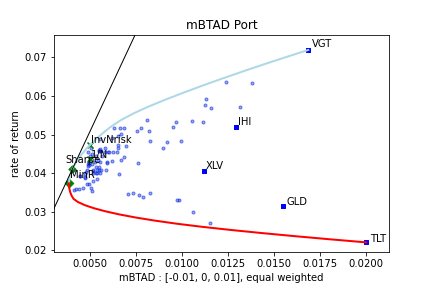
\includegraphics[width=.95\linewidth]{../figs/mBTADFrontier1.png}
  \caption{Rate of return vs. \mBTAD}
  \label{BTAD_fig1a}
\end{subfigure}%
\begin{subfigure}{.5\textwidth}
  \centering
  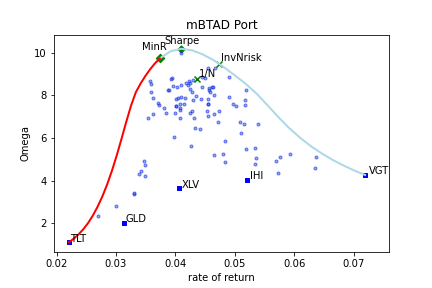
\includegraphics[width=.95\linewidth]{../figs/mBTADFrontier2.png}
  \caption{Omega vs. rate of return}
  \label{BTAD_fig1b}
\end{subfigure}
\caption{\mBTAD\ : [$\alpha=(-0.01, 0.0, 0.01)$, equal weighted] frontiers.}
\label{BTAD_fig1}
\end{figure}

\BackToContents

\subsubsection{Backtesting Omega optimal portfolio}

Here is an example, using \azapy\ package, of computing a portfolio backtesting.
For this example, we have chosen a portfolio quarterly rebalanced according
to the maximization of Omega ratio. At each rebalancing date,
the portfolio weights
are calibrated based on 3.25 years of prior historical market data.

Other rebalancing strategies can be considered
by changing the value of {\it rtype} parameter in the call of {\it set\_model} function below.
For more details see the package documentation at \azapydoc.

\lstinputlisting[language=Python]{../PyScripts/BTAD_Port.py}

\begin{figure}[H]
    \centering
    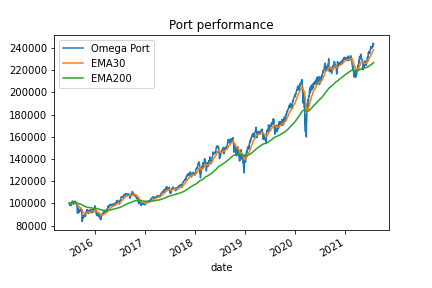
\includegraphics[width=.95\linewidth]{../figs/Port_mBTAD_Sharpe.png}
    \caption{Backtesting of quarterly rebalanced Omega optimal portfolio for
    \mBTAD\ : [$\alpha=(-0.01, 0.0, 0.01)$, equal weighted].}
    \label{BTAD_Port_fig}
\end{figure}


\BackToContents




\subsection{mBTSD-based optimization strategies}\label{S:mBTSD}

\BTSD\ stands for Below Threshold Semi-Deviation.
It is the square root of below threshold semi-variance proposed by Markowitz in 1959 \cite{Markowitz2}.
In contrast to standard deviation, \BTSD\ takes in account only the downside events below a prespecified threshold.

Its mathematical expression is given by $\BTM^{(p)}$, from Eq.~(\ref{btm1}), for $p=2$, \ie,
\begin{equation}
    \BTSD_\alpha = \left\| \left( \alpha - r \right)^+ \right\|_2,
    \label{btsd01}
\end{equation}
where $\alpha$ is the threshold level and $\|\cdot\|_2 = (\mE[|\cdot |^2])^{1/2}$ is the $L^2$-norm.
Note that \BTSD\ is the $L_2$ version of \BTAD.

\BTSD\ has gained more attention after the introduction of
Sortino ratio in 1994 by Sortino and Price \cite{Sortino} (see also \cite{Kaplan}).

Sortino ratio is defined as
\begin{equation}
    \Sortino_\alpha = \frac{\mE[r] - \alpha}{\BTSD_\alpha},
    \label{btsd02}
\end{equation}
and is equivalent to \BTSD-Sharpe ratio for $\mu_0 = \alpha$.
In contrast to the Sharpe ratio, Sortino ratio measures the expected excess returns 
per unit of downside risk of realizations below a predefined threshold.

As we mentioned in the preamble of this section, \BTSD\ can be defined in terms of both standard rate of return, $r$, and
detrended rate of return, $\br = r - \mE[r]$. In this subsection we will use the latter specification to express mathematical formulas.
However, we should keep in
mind that, switching between the \BTSD\ definitions, is a simple matter of replacing $\br$ with $r$.\footnote{The \azapy\ package provides a logical
flag to switch between the use of $r$ and $\br$ (see \azapydoc).}

Like \mBTAD\ from Eq.~(\ref{btm2}), \BTSD\ can be extended to a mixture, \ie,
\begin{equation}
    \mBTSD = \sum_{l=1}^L \cK_l \times \BTSD_{\alpha_l},
    \label{btsd0}
\end{equation}
where $\{\cK_l\}_{l=1,\cdots,L}$ is a set of positive coefficients normalized to unit (the mixture coefficients) and
$\{\alpha_l\}_{l=1,\cdots,L}$ is a set of distinct thresholds.

We will refer to the \mBTSD-Sharpe ratio as Sortino ratio since Sortino ratio terminology is more popular among practitioners. However,
we should keep in mind that our Sortino ratio definition is equivalent to the original Sortino and Price \cite{Sortino}
definition only in the case where $L=1$ and $\alpha_1 = \mu_0$ with standard rate of return.

Like \mBTAD, \mBTSD\ is not a genuine dispersion measure. It violates the positive homogeneity axiom and, in the case where standard rates of return
are used, it also violates local invariance. An exception is the case where $L=1$ and $\alpha_1=0$ with detrended rates of return.
In this case, $\BTSD_0$ is equivalent to the first order \mLSD, delta-risk $\delta^{(2)}_1$ from Eq.~(\ref{LSD02}), which is a genuine dispersion measure.

\BackToContents


\subsubsection{mBTSD dispersion measure}
The computation of \mBTSD\ is straightforward. Given a set $\{r_i\}_{i=1,\cdots,N}$ of observed rates or returns, we have
\begin{equation}
    \BTAD_\alpha = \left( \frac{1}{N}\sum_{i=1}^N \left[ \left(\alpha - \br_i \right)^+ \right]^2 \right)^{1/2}.
    \label{btsd1}
\end{equation}
Then, \mBTSD\ is given by the sum from Eq.~(\ref{btsd0}).

\BackToContents

\subsubsection{mBTSD optimal portfolio}
The optimization is described by Eqs.~(\ref{gg1}) from Sec.~\ref{strategies} point~\ref{OptRisk},
where $\rho$ is given by $\mBTSD$ from Eq.~(\ref{btsd0}).
It is the following SOCP problem.

\bigskip
\noindent Minimize over $\{\{w_k\}_{k=1,\cdots,M}, \{ \eta_l, \{ s_{li} \}_{i=1,\cdots,N} \}_{l=1,\cdots,L} \}$,
\begin{subequations}\label{btsd2}
\begin{align}
    &g = \sum_{l=1}^L \cK_l \eta_l, \label{btsd2a} \\
    \st &\left( \frac{1}{N} \sum_{i=1}^N s_{li}^2 \right)^{1/2} \leq \eta_l, \label{btsd2b} \\
    & s_{li} + \sum_{k=1}^M w_k \br_{ki} \geq \alpha_l, \label{btsd2c} \\
    & \sum_{k=1}^M w_k \mu_k \geq \mu, \label{btsd2d} \\
    & \sum_{k=1}^M w_k = 1, \label{btsd2e} \\
    & s_{li} \geq 0, \label{btsd2g} \\
    & \eta_l \geq 0, \label{btsdg} \\
    & w_k \geq 0, \label{btsd2f}
\end{align}
\end{subequations}

\noindent where $\mu$, in Eq.~(\ref{btsd2d}), is the portfolio targeted expected rate of return, while $\mu_k$ for $k = 1,\cdots,M$
are the portfolio components expected rate of returns.
Then, we have
\begin{subequations}\label{btsd3}
\begin{align}
    \RR &= \sum_{k=1}^M w_k^* \mu_k, \label{btsd3a} \\
    \mBTSD &= g^*, \label{btsd13b} \\
    \BTSD_{\alpha_l} &= \eta_l^*, \label{btsd3c}
\end{align}
\end{subequations}

\noindent where $^*$ denotes the solution of  SOCP problem.
In addition to the optimal portfolio weights $\{w_k^*\}_{k=1,\cdots,M}$ and
expected rate of return $\RR$, the
SOCP solution provides information about the portfolio \mBTSD\ and its components.

\bigskip
\noindent Here is an example, using the \azapy\ package, of how to compute the \mBTSD\ optimal portfolio.
The \mBTSD\ time horizon was set to one quarter and the calibration is performed using the prior 3.25 years of
close-adjusted historical prices (default settings).
For more details see the package documentation at \azapydoc.

\lstinputlisting[language=Python]{../PyScripts/BTSD_RiskOptim.py}

\BackToContents


\subsubsection{Minimum mBTSD portfolio}

Following the result from Sec.~\ref{strategies} point~\ref{MinRisk},
the algorithm to compute the optimal portfolio with minimum \mBTSD\ is given by Eqs.~(\ref{btsd1}) where
$\mu$ from r.h.s. of Eq.~(\ref{btsd2d}) is set to a value equal to the smallest expected rate of
return among the portfolio components, \ie\ $\mu=\min_k\{\mu_k\}$.

\bigskip
\noindent Here is an example, using the \azapy\ package, of how to compute the minimum \mBTSD\ portfolio.
The \mBTSD\ time horizon was set to one quarter and the calibration is performed using the prior 3.25 years of
close-adjusted historical prices (default settings).
For more details see the package documentation at \azapydoc.

\lstinputlisting[language=Python]{../PyScripts/BTSD_MinRisk.py}

\BackToContents


\subsubsection{mBTSD optimal portfolio for targeted risk value}
This optimization is described by Eqs.~(\ref{gg2}) from Sec.~\ref{strategies} point~\ref{TargetRisk},
where $\rho$ is given by \mBTSD\ from Eq.\ (\ref{btsd0}).
It is the following SOCP problem.

\bigskip
\noindent Maximize over $\{\{w_k\}_{k=1,\cdots,M}, \{ \eta_l, \{ s_{li} \}_{i=1,\cdots,N} \}_{l=1,\cdots,L} \}$,
\begin{subequations}\label{btsd4}
\begin{align}
    &g = \sum_{k=1}^M w_k \mu_k, \label{btsd4a} \\
    \st & \left( \frac{1}{N}  \sum_{i=1}^N s_{li}^2 \right)^{1/2} \leq \eta_l, \label{btsd4c} \\
    & s_{li} + \sum_{k=1}^M w_k \br_{ki} \geq \alpha_l, \label{btsd4d} \\
    & \sum_{l=1}^L \cK_l \eta_l = \mBTSD_0, \label{btsd4b} \\
    & \sum_{k=1}^M w_k = 1, \label{btsd4e} \\
    & s_{li} \geq 0, \label{btsd4g} \\
    & \eta_l \geq 0, \label{btsd4h} \\
    & w_k \geq 0, \label{btsd4f}
\end{align}
\end{subequations}

\noindent where $\mBTSD_0$ in Eq.~(\ref{btsd4b}) is the portfolio targeted \mBTSD\ dispersion value.
Then, we have
\begin{subequations}\label{btsd5}
\begin{align}
    \RR &= g^*, \label{btsd5a} \\
    \BTSD_{\alpha_l} &= \eta_l^*, \label{btsd5b}
\end{align}
\end{subequations}

\noindent where the superscript $^*$ denotes the solution of SOCP problem.
In addition to the optimal portfolio weights $\{w_k^*\}_{k=1,\cdots,M}$ and expected rate of return $\RR$,
the SOCP solution provides information about \mBTSD\ and its components,
although, this information is likely to be known at the outset.

\bigskip
\noindent Here is an example, using the \azapy\ package, of how to compute the optimal portfolio
with the same \mBTSD\ as the equal weighted portfolio.
The \mBTSD\ time horizon was set to one quarter and the calibration is performed using the prior 3.25 years of
close-adjusted historical prices (default settings).
For more details see the package documentation at \azapydoc.

\lstinputlisting[language=Python]{../PyScripts/BTSD_InvNrisk.py}

\BackToContents


\subsubsection{mBTSD optimal portfolio for fixed risk-aversion factor}
This optimization is described by Eqs.~(\ref{gg3}) from Sec.~\ref{strategies} point~\ref{RiskAverse},
where $\rho$ is given by \mBTSD\ from Eq.~(\ref{btsd0}).
It is the following LP problem.

\bigskip
\noindent Maximize over $\{\{w_k\}_{k=1,\cdots,M}, \{ \eta_l, \{ s_{li} \}_{i=1,\cdots,N} \}_{l=1,\cdots,L} \}$,
\begin{subequations}\label{btsd6}
\begin{align}
    &g = \sum_{k=1}^M w_k \mu_k - \lambda \sum_{l=1}^L \cK_l \eta_l, \label{btsd6a} \\
    \st & \left( \frac{1}{N}  \sum_{i=1}^N s_{li}^2 \right)^{1/2} \leq \eta_l, \label{btsd6b} \\
    & s_{li} + \sum_{k=1}^M w_k \br_{ki} \geq \alpha_l, \label{btsd6c} \\
    & \sum_{k=1}^M w_k = 1, \label{btsd6d} \\
    & s_{li} \geq 0, \label{btsd6f} \\
    & \eta_l \geq 0, \label{btsd6g} \\
    & w_k \geq 0, \label{btsd6e}
\end{align}
\end{subequations}

\noindent where $\lambda$ from Eqs.~(\ref{btsd6a}) is the risk-aversion factor.
Then, we have
\begin{subequations}\label{btsd7}
\begin{align}
    \RR &= \sum_{k=1}^M w_k^* \mu_k, \label{btsd7a} \\
    \mBTSD &= \frac{\RR - g^*}{\lambda}, \label{btsd7b} \\
    \BTSD_{\alpha_l} &= \eta_l^*, \label{btsd7c}
\end{align}
\end{subequations}

\noindent where the superscript $^*$ denotes the solution of SOCP problem.
In addition to the optimal portfolio weights $\{w_k^*\}_{k=1,\cdots,M}$ and expected rate of return $\RR$,
the SOCP solution provides information about \mBTSD\ and its \BTSD\ components values.

\bigskip
\noindent Here is an example, using the \azapy\ package, of how to compute the optimal portfolio
for a given value of the risk-aversion factor $\lambda$.
The \mBTSD\ time horizon was set to one quarter and the calibration is performed using the prior 3.25 years of
close-adjusted historical prices (default settings).
For more details see the package documentation at \azapydoc.

\lstinputlisting[language=Python]{../PyScripts/BTSD_Averse.py}

\BackToContents


\subsubsection{Sortino optimal portfolio - maximization solution}
This optimization targets the maximization of Sortino ratio. It is based on the
Eqs.~(\ref{gg4}) from Sec.~\ref{strategies} point~\ref{MaxSharpe}, where $\rho$ is given by \mBTSD\ from Eq.~(\ref{btsd0}).
The optimization can be formulated as an SOCP problem
if Eq.\ (\ref{gg4b}) can be expressed as a second order cone constraint. This can be achieved by
introducing the variable transformations $\bw_k = t w_k$, $\bs_{li} = t s_{li}$ and $\bbeta_l = t \eta_l$.
Then, the SCOP problem can be written as follows.

\bigskip
\noindent Maximize over $\{\{\bw_k\}_{k=1,\cdots,M}, \{ \bbeta_l, \{ \bs_{li} \}_{i=1,\cdots,N} \}_{l=1,\cdots,L}, t \}$,
\begin{subequations}\label{btsd8}
\begin{align}
    &g = \sum_{k=1}^M \bw_k \mu_k - \mu_0 t, \label{btsd8a} \\
    \st &\left( \frac{1}{N}  \sum_{i=1}^N \bs_{li}^2 \right)^{1/2} \leq \bbeta_l, \label{btsd8c} \\
    &\bs_{li}  + \sum_{k=1}^M \bw_k \br_{ki} - \alpha_l t \geq 0, \label{btsd8d} \\
    &\sum_{l=1}^L \cK_l \bbeta_l = 1, \label{btsd8b} \\
    &\sum_{k=1}^M \bw_k - t = 0, \label{btsd8e} \\
    &t \geq 0, \label{btsd8h} \\
    &\bs_{li} \geq 0, \label{btsd8g} \\
    &\bbeta_l \geq 0, \label{btsd8i} \\
    &\bw_k \geq 0, \label{btsd8f}
\end{align}
\end{subequations}

\noindent where $\mu_0$ in Eqs.~(\ref{btsd8a}) is the
risk-free rate accessible to the investor.
Then, we have
\begin{subequations}\label{btsd9}
\begin{align}
    w_k &= \frac{\bw_k^*}{t^*} , \label{btsd9a} \\
    \RR &= \frac{g^*}{t^*} + \mu_0, \label{btsd9c} \\
    \Sortino &= g^*, \label{btsd9b} \\
    \mBTSD &= \frac{1}{t^*}, \label{btsd9d} \\
    \BTSD_{\alpha_l} &= \frac{\bbeta_l^*}{t^*}, \label{btsd9e}
\end{align}
\end{subequations}

\noindent where $^*$ denotes the solution of SOCP problem.
In addition to the optimal portfolio weights $\{w_k\}_{k=1,\cdots,M}$, expected rate of return $\RR$ and
Sortino ratio $\Sortino$,
the SOCP solution provides information about \mBTSD\ and its components.

\bigskip
\noindent Here is an example, using the \azapy\ package, of how to compute the Sortino optimal portfolio using the maximization
of Sortino ratio.
The \mBTSD\ time horizon was set to one quarter and the calibration is performed using the prior 3.25 years of
close-adjusted historical prices (default settings).
For more details see the package documentation at \azapydoc.

\lstinputlisting[language=Python]{../PyScripts/BTSD_Sharpe.py}

\BackToContents


\subsubsection{Sortino optimal portfolio - minimization solution}
This optimization targets the minimization of the inverse of Sortino ratio.
It is described by Eqs.~(\ref{gg8}) from Sec.~\ref{strategies} point~\ref{MinSharpe}, where
$\rho$ is given by \mBTSD\ from Eq.~(\ref{btsd0}).
The optimization can be formulated as an SOCP problem if Eq.~(\ref{gg8a}) can  be expressed as a second order cone constraint. This can be achieved by
introducing the variable transformations
$\bw_k = t w_k$, $\bs_{li} = t s_{li}$ and $\bbeta_l = t \eta_l$.
Then, the SOCP problem can be written as follows.

\bigskip
\noindent Minimize over $\{ \{\bw_k\}_{k=1,\cdots,M}, \{ \bbeta_l, \{ \bs_{li} \}_{i=1,\cdots,N} \}_{l=1,\cdots,L}, t \}$
\begin{subequations}\label{btsd10}
\begin{align}
    &g = \sum_{l=1}^L \cK_l \bbeta_l, \label{btsd10a} \\
    \st &\left( \frac{1}{N}  \sum_{i=1}^N \bs_{li}^2 \right)^{1/2} \leq \bbeta_l, \label{btsd10b} \\
    &\bs_{li}  + \sum_{k=1}^M \bw_k \br_{ki} - \alpha_l t \geq 0, \label{btsd10c} \\
    &\sum_{k=1}^M \bw_k \mu_k -\mu_0 t = 1, \label{btsd10d} \\
    &\sum_{k=1}^M \bw_k - t = 0, \label{btsd10e} \\
    &t \geq 0, \label{btsd10h} \\
    &\bs_{li} \geq 0, \label{btsd10g} \\
    &\bbeta_l \geq 0, \label{btsd10i} \\
    &\bw_k \geq 0, \label{btsd10f}
\end{align}
\end{subequations}

\noindent where $\mu_0$ in Eqs.~(\ref{btsd8a}) is the
risk-free rate accessible to the investor.
Then, we have
\begin{subequations}\label{btsd11}
\begin{align}
    w_k &= \frac{\bw_k^*}{t^*} , \label{btsd11a} \\
    \RR &= \frac{1}{t^*} + \mu_0, \label{btsd11c} \\
    \Sortino &= \frac{1}{g^*}, \label{btsd11b} \\
    \mBTSD &= \frac{g^*}{t^*}, \label{btsd11d} \\
    \BTSD_{\alpha_l} &= \frac{\bbeta_l^*}{t^*}, \label{btsd11e}
\end{align}
\end{subequations}

\noindent where $^*$ denotes the solution of SOCP problem.
In addition to the optimal portfolio weights $\{w_k\}_{k=1,\cdots,M}$, expected rate of return $\RR$ and
Sortino ratio \Sortino,
the SOCP solution provides information about \mBTSD\ and its \BTSD\ components.

\bigskip
\noindent Here is an example, using the \azapy\ package, of how to compute the Sortino optimal portfolio using the minimization
of the inverse of Sortino ratio.
The \mBTSD\ time horizon was set to one quarter and the calibration is performed using the prior 3.25 years of
close-adjusted historical prices (default settings).
For more details see the package documentation at \azapydoc.

\lstinputlisting[language=Python]{../PyScripts/BTSD_InvSharpe.py}

\BackToContents


\subsubsection{mBTSD frontiers}

Here is an example of how to compute the \mBTSD\ frontiers using the \azapy\
package. The \mBTSD\ time horizon was set to one quarter and the calibration is performed using the prior 3.25 years of
close-adjusted historical prices (default settings).
For more details see the package documentation at \azapydoc.

The script will produce the plots in Figs.~\ref{BTSD_fig1a} and \ref{BTSD_fig1b}
for historical data collected up to 2021-07-27.

\lstinputlisting[language=Python]{../PyScripts/BTSD_frontiers.py}

\begin{figure}[H]
\centering
\begin{subfigure}{.5\textwidth}
  \centering
  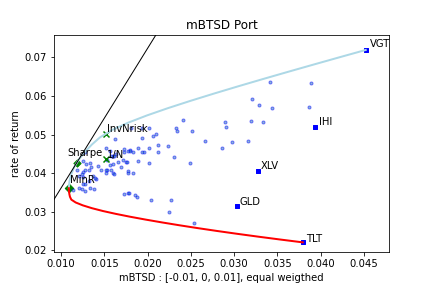
\includegraphics[width=.95\linewidth]{../figs/mBTSDFrontier1.png}
  \caption{Rate of return vs. \mBTSD}
  \label{BTSD_fig1a}
\end{subfigure}%
\begin{subfigure}{.5\textwidth}
  \centering
  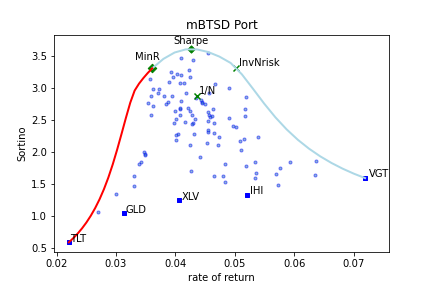
\includegraphics[width=.95\linewidth]{../figs/mBTSDFrontier2.png}
  \caption{Sortino vs. rate of return}
  \label{BTSD_fig1b}
\end{subfigure}
\caption{\mBTSD\ : [$\alpha=(-0.01, 0.0, 0.01)$, equal weighted] frontiers.}
\label{BTSD_fig1}
\end{figure}

\BackToContents


\subsubsection{Backtesting Sortino optimal portfolio}

Here is an example, using \azapy\ package, of computing a portfolio backtesting.
For this example, we have chosen a portfolio quarterly rebalanced according
to the maximization of Sortino ratio. At each rebalancing date,
the portfolio weights
are calibrated based on 3.25 years of prior historical market data.

Other rebalancing strategies can be considered
by changing the value of {\it rtype} parameter in the call of {\it set\_model} function below.
For more details see the package documentation at \azapydoc.

\lstinputlisting[language=Python]{../PyScripts/BTSD_Port.py}

\begin{figure}[H]
    \centering
    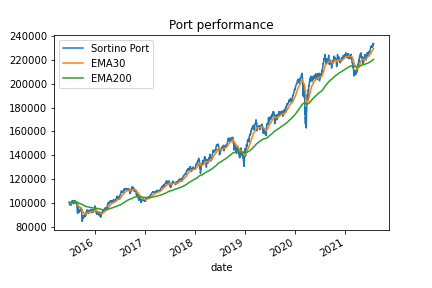
\includegraphics[width=.95\linewidth]{../figs/Port_mBTSD_Sharpe.png}
    \caption{Backtesting of quarterly rebalanced Sortino optimal portfolio,
    \mBTSD\ : [$\alpha=(-0.01, 0.0, 0.01)$, equal weighted].}
    \label{BTSD_Port_fig}
\end{figure}

\BackToContents
 